\section{Exercise 1: Satellite galaxies}

In this section, the solutions to the first exercise are presented. 

Our script is given by:
\lstinputlisting[language=Python]{Satellites.py}

\subsection{1a. Finding A by numerical integration.}
In order to find the normalization constant A in the formula given in the problem sheet, we implemented a Romberg integration algorithm. For the integral, we use $dV = 4\pi r^2 dr$. For the rest of this exercise, $n(x)$ will refer to the number density, and $N(x)$ will be the number density multiplied by $ 4\pi r^2$. The relevant code is given below:

\lstinputlisting[language=Python, firstline=4, lastline=67]{Satellites.py}

As can be seen in the code above, romberg\_interval calculates the integral between a and b up to some order, and romberg then sums this over many intervals. In this case, we go up to order 10, where we use 15 function evaluations. The output given by this piece of the code is given below. For the sanity check, we calculate the integral again with our calculated value of A, and we see that it is equal to one.

\lstinputlisting[firstline=1, lastline=2]{satellite_output.txt}

\subsection{1b. Generating satellite positions}
For this subquestion, we made use of rejection sampling in log space to sample 10,000 points following the analytical distribution $N(x)dx / \langle N_{sat} \rangle$. The relevant code is given below.

\lstinputlisting[language=Python, firstline=69, lastline=188]{Satellites.py}

The analytical function is equal to $N(x) = n(x) 4\pi r^2$. We first find the maximum this function takes on in our interval, by evaluating the function at many points (which is already necessary for plotting), sorting the array of evaluations, and finding the first element of it. We use this maximum as the maximum for our uniform random numbers.

Speaking of uniform random numbers, we generate ours as follows: we feed a number into a xor\_shift algorithm, and the result of that is put into a Multiply With Carry random number generator. The MWC returns both a number and a state: the number is output as a random number, and the state is then fed back into the xor\_shift algorithm, where the next random number will be generated. This of course generates integers between 0 and $2^{32}$, so we use the rng\_float function to generate uniform random floats between two values.

We use rejection sampling to sample the distribution, and we do so by sampling our x value in log space, to match the logarithmic bins given by the exercise instructions. We then compare another random number $y = U(0, max)$, with max being the maximum calculated earlier, to the function evaluated at our x value. If y is smaller than x, we accept y as part of our sample. We generate samples until we've reached 10,000, at which point we stop generating them.

The result of this sampling is plotted below. Note that we normalize our histogram by dividing by the total amount of samples generated to reach 10,000 accepted samples, and multiplying by the average number of satellites.

\begin{figure}[h!]
\label{fig:1b}
\caption{In red, the analytical distribution that we are supposed to sample from is plotted. The blue bars correspond to the logarithmic bins given, and their heights are the number of samples per bin. The bars follow the distribution nicely.}
\centering

\includegraphics[width=0.7\textwidth]{my_solution_1b.png}
\end{figure}

\subsection{1c. Random galaxy selection}
In this subquestion, we randomly select satellite galaxies from the sample in b in a way that selects every galaxy with equal probability, does not draw the same galaxy twice, and does not reject any draw. The relevant code is included here. All sorting in this exercise is done with mergesort, which can be found in the first code snippet in this exercise.

\lstinputlisting[language=Python, firstline=189, lastline=207]{Satellites.py}

We achieve this by generating an array of 10,000 random numbers, and sorting them to create a random sorting index. We then apply this sorting index to the random sample from b, and select the first 100 elements. This achieves the requirements specified above. 

Then, we sort the 100 galaxies from smallest to largest radius using our implementation of mergesort, and plot the number of galaxies within a radius. 

\begin{figure}[h!]
\label{fig:1c}
\caption{We see that the number of galaxies within a radius is strictly increasing, which means the array is sorted correctly.}
\centering
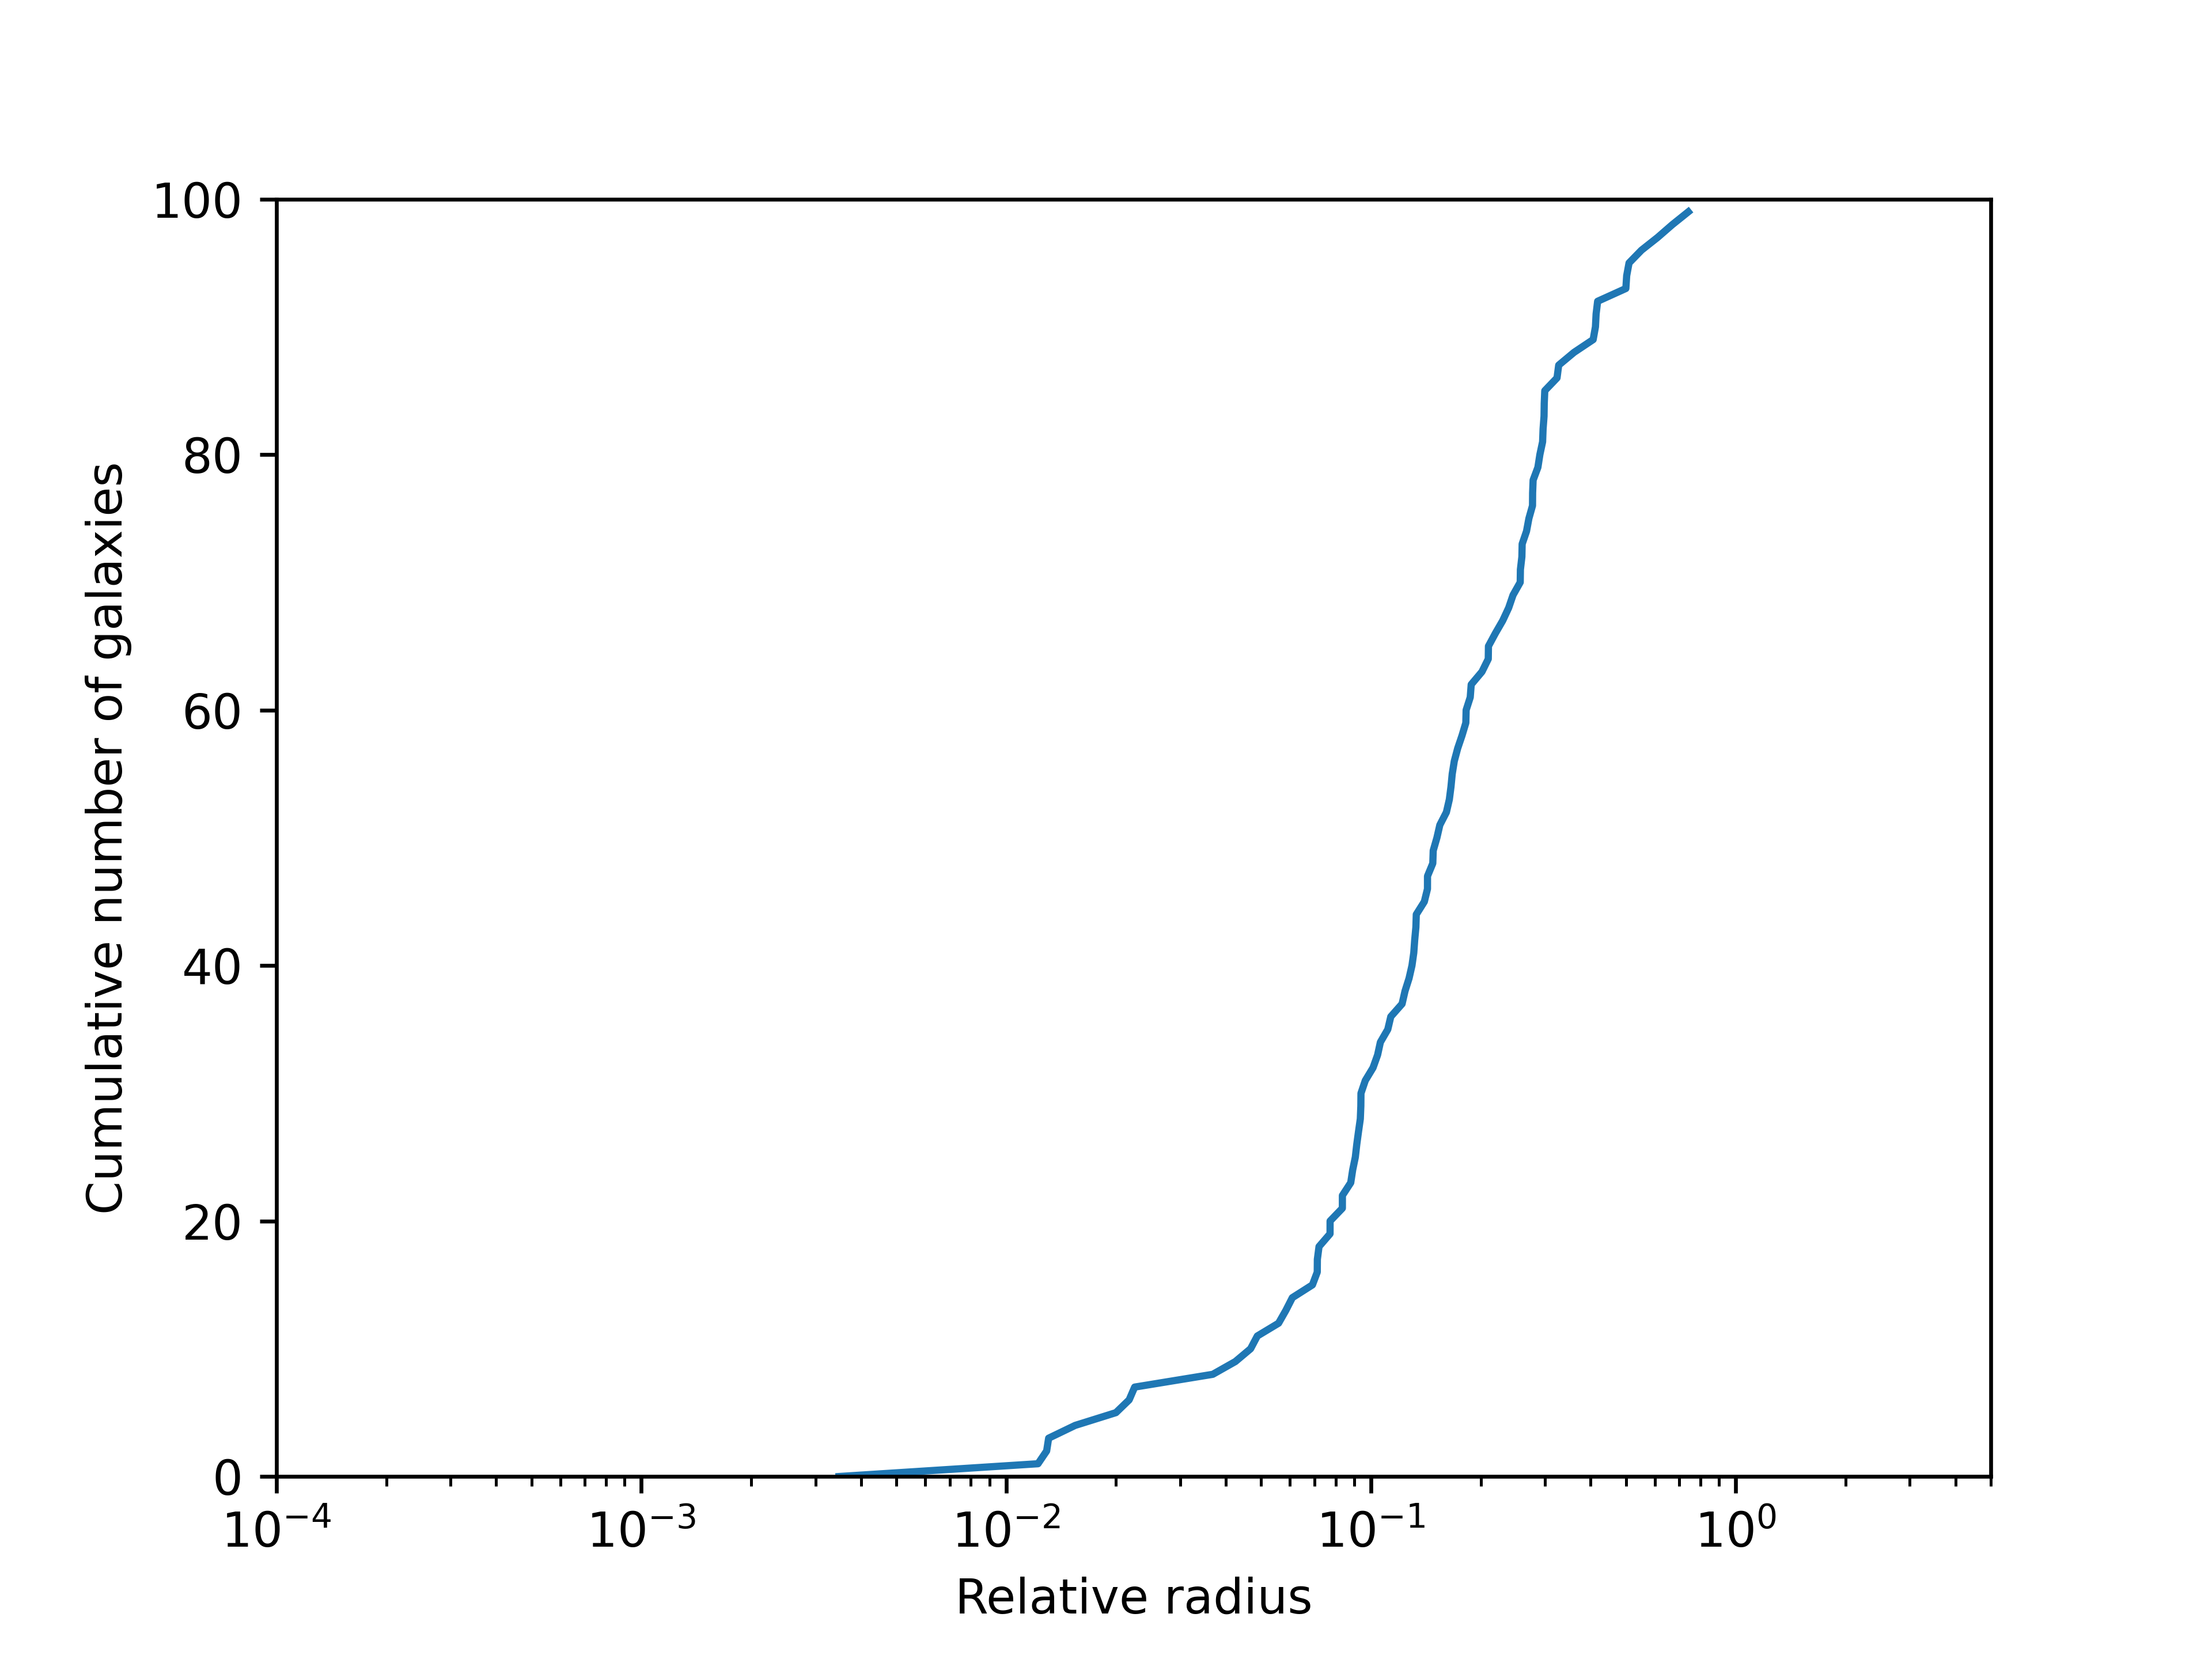
\includegraphics[width=0.7\textwidth]{my_solution_1c.png}
\end{figure}

\subsection{1d. Derivative of n(x)}
In this section, we calculate the derivative $d n(x)/dx$ at $x=1$ numerically. We used Ridder's algorithm to find the derivative, as seen in the code below.

\lstinputlisting[language=Python, firstline = 209, lastline = 240]{Satellites.py}

The output is given here:

\lstinputlisting[firstline=3, lastline = 5]{satellite_output.txt}









